% !TEX root = MasterPaper.tex
\chapter{臨場感を演出する集団ロボットの内部モデル}
\thispagestyle{fancy} % このページのみ
\lhead{}
\chead{}
\rhead{}
\lfoot{} 
\cfoot{\thepage}  
\rfoot{}
%

\section{IECシステムの概要}
\label{sec3.1}


本研究では,性格特性を表現するジェスチャをIECを用いて最適化するシステムを提案する.本システムでは,提示評価フェーズと最適化フェーズの二段階で構成される.提示評価フェーズでは,システムはユーザに対して,二体のロボットを順に提示する.提示する際,ロボットはスクリプトを読み上げながら,ビートジェスチャを行う.そして,ユーザは提示された2体のロボットを一対比較する.この流れを一定数繰り返す.最適化フェーズでは,提示フェーズで得たユーザの嗜好情報に基づいてロボットジェスチャを最適化する.

本節では,本システムに関する評価,最適化,遺伝子表現について述べる.



\subsection{ロボットジェスチャの評価手法}
\label{sec3.1.1}    

本研究では,評価手法として,トーナメント式評価手法を用いた.図○○にトーナメント式評価手法による解評価法を示す.まず,IGAの処理において初めに生成される解候補を,ランダムにトーナメント表に配置する.ランダムに配置された解候補をp1~p8とする.次に,トーナメント表の対戦組み合わせに基づいて,ユーザは対戦する2つの解候補を一対比較によって評価し,優劣を判定する.決勝戦まで対戦が終了すると,勝ち上がった対戦数に応じて各解候補に評価点を付与する.




まず,同一世代に生成された個体をランダムでトーナメント表に配置する.そして,ユーザが対戦する個体の相対評価を行い,対戦個体の優劣を決定する.





何を評価するのか 遺伝子表現でかく?




\subsection{ロボットジェスチャの最適化}
\label{sec3.1.2}


本節では,最適化について述べる.

提案システムのフローチャートを図○○に示す.


\subsection{ロボットジェスチャの遺伝子表現}
\label{sec3.1.3}
GAを用いてロボットジェスチャの最適化をするために,ロボットジェスチャを遺伝子として表現する.

本研究では,


\newpage

\section{実験環境}
\label{sec3.2}

実環境でのインタラクションにおいて,感情を表出するロボット集団を準備することや,リアルタイムでの勝利確率を取得することは困難であるため,本実験では仮想環境であるVR空間を用いて実験を行う.本研究では,採用しているバーチャルアバターをロボットと呼ぶ.ロボット集団と共に野球観戦を行うため,スポーツバーを模した空間をゲームエンジンであるUnityを用いて制作している\cite{unity}.

本実験では,観戦を行う場所としてスポーツバーを模した内装と,感情を表出するロボット集団を,Unity内のAsset storeにある有償のAssetを改変して使用している\cite{bar}\cite{lilrobot}.スポーツバーとロボット集団の外観を図\ref{sports_bar},図\ref{robot}に示す.

また,Unityで作成したVR空間を体験するためのデバイスとして,ヘッドマウントディスプレイ,ヘッドフォンを使用する.この機器は家庭用VRデバイスであるHTC VIVEを用いる\cite{vive}.

本実験で使用するヘッドフォン付きヘッドマウントディスプレイを図\ref{Vive}に示す.


\vspace{1cm}
 \begin{figure}[H]
 \begin{center}
  \centering
  \includegraphics[width=15cm]{images/chapter3/sports_bar.eps}
  \caption{実験環境}
  \label{sports_bar}
 \end{center}
\end{figure}


\newpage

\vspace{1cm}
 \begin{figure}[!h]
 \begin{center}
  \centering
  \includegraphics[width=15cm]{images/chapter3/robot.eps}
  \caption{ロボット集団}
  \label{robot}
 \end{center}
\end{figure}


\vspace{1cm}
 \begin{figure}[!h]
 \begin{center}
  \centering
  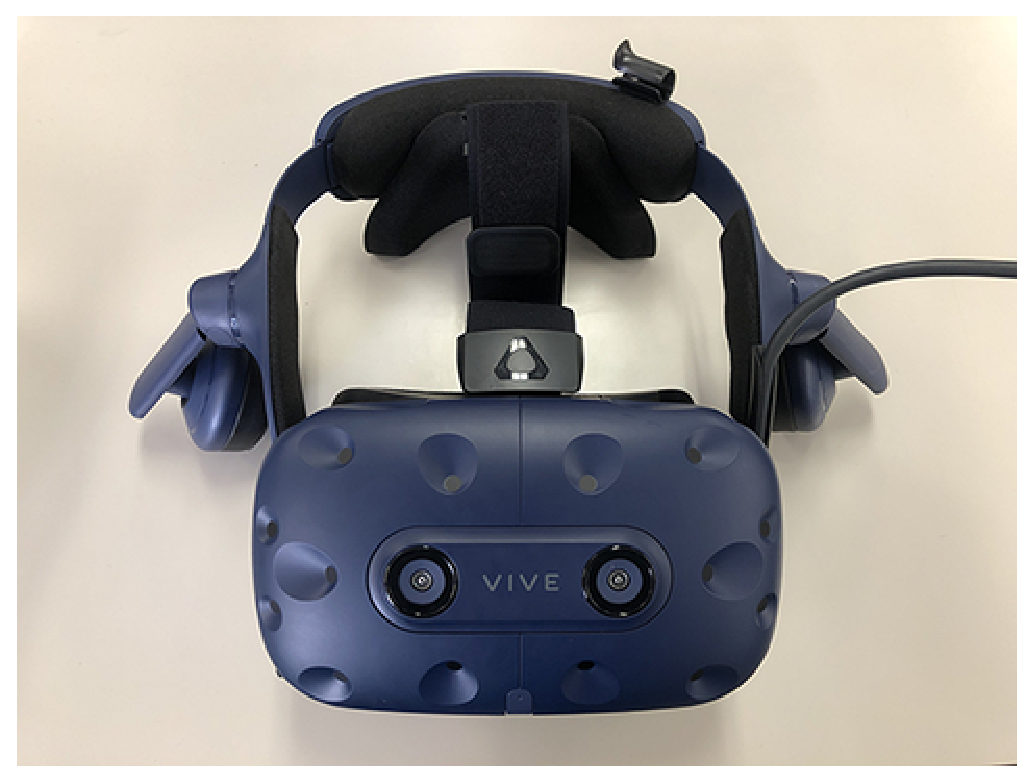
\includegraphics[width=12cm]{images/chapter3/Vive.eps}
  \caption{ヘッドマウントディスプレイ}
  \label{Vive}
 \end{center}
\end{figure}


\subsection{スポーツバーでの観戦}
\label{sec3.2.1}

実験中の画面の様子を図\ref{bar_scene}に示す.本実験では被験者とロボットのみで試合観戦を行う.共に試合観戦を行うロボット集団は,スポーツバーを模した空間上の席に着席して試合観戦を行う.

被験者はヘッドフォン付きヘッドマウントディスプレイを装着して着席し,その場から動かずにロボット集団と試合観戦を行う.図\ref{sports_bar}の前方にある4台のモニターに映し出される試合を観戦する.また,ヘッドマウントディスプレイによる映像だけでなく,ヘッドフォンからは観戦映像の音が流れている.このように,被験者は視覚情報と聴覚情報の2つを用いて試合観戦を行う.




\vspace{1cm}
 \begin{figure}[!h]
 \begin{center}
  \centering
  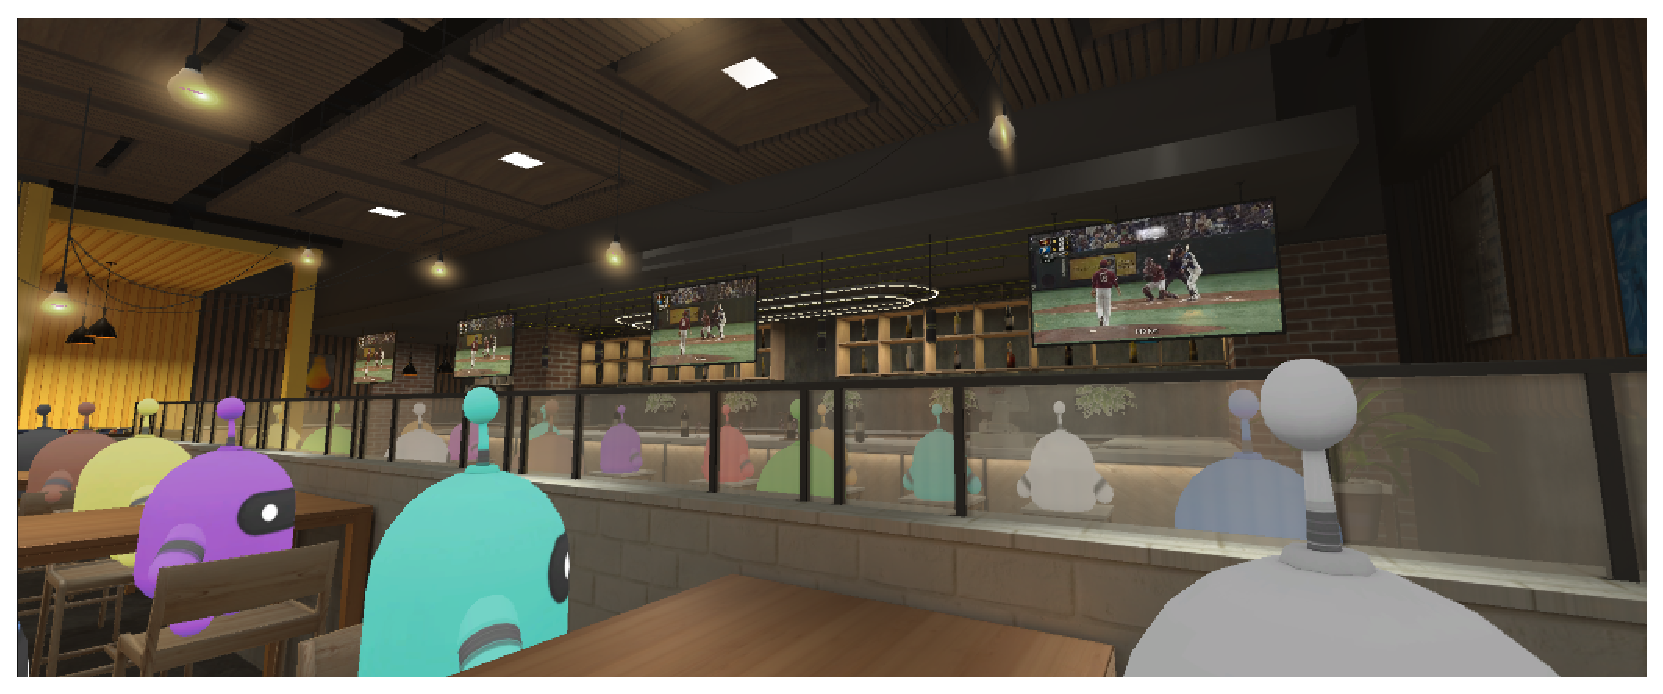
\includegraphics[width=15cm]{images/chapter3/bar_scene.eps}
  \caption{スポーツバーの様子}
  \label{bar_scene}
 \end{center}
\end{figure}



\newpage



\subsection{ロボット集団の動作}
\label{sec3.2.2}

被験者と共に試合観戦をするロボット集団は,感情表出しない状態(Idle状態),喜の感情表出,哀の感情表出を行う.

Idle状態では,ロボットは図\ref{Idle}の状態から,一定の周期でゆっくりと上下に反復運動を行う.この動作によって,人間の呼吸運動を再現する.また,各ロボットは,反復運動の速さを24回/分,27回/分,30回/分,33回/分,36回/分の5種類からランダムで設定されており,速さを変えることによってロボットの個性を設計している.

喜の感情表出は,図\ref{happy}のように,手を挙げながらジャンプする動作を繰り返すことで表出する.表出する感情の程度は,ジャンプする動作の速さを変更することで設計する.本実験では感情の程度を小,中,大の3種類に設定し,小なら30回/分,中なら50回/分,大なら70回/分の速さで感情表出を行う.

哀の感情表出は,図\ref{sad}のように,飛び上がって倒れこむ動作を繰り返すことで表出する.表出する感情の程度は,倒れこむ速さを変更することで設計する.喜の感情と同じく3段階の感情の程度を設定し,小なら12回/分,中なら15回/分,大なら20回/分の速さで感情表出を行う.


\vspace{1cm}
 \begin{figure}[!h]
 \begin{center}
  \centering
  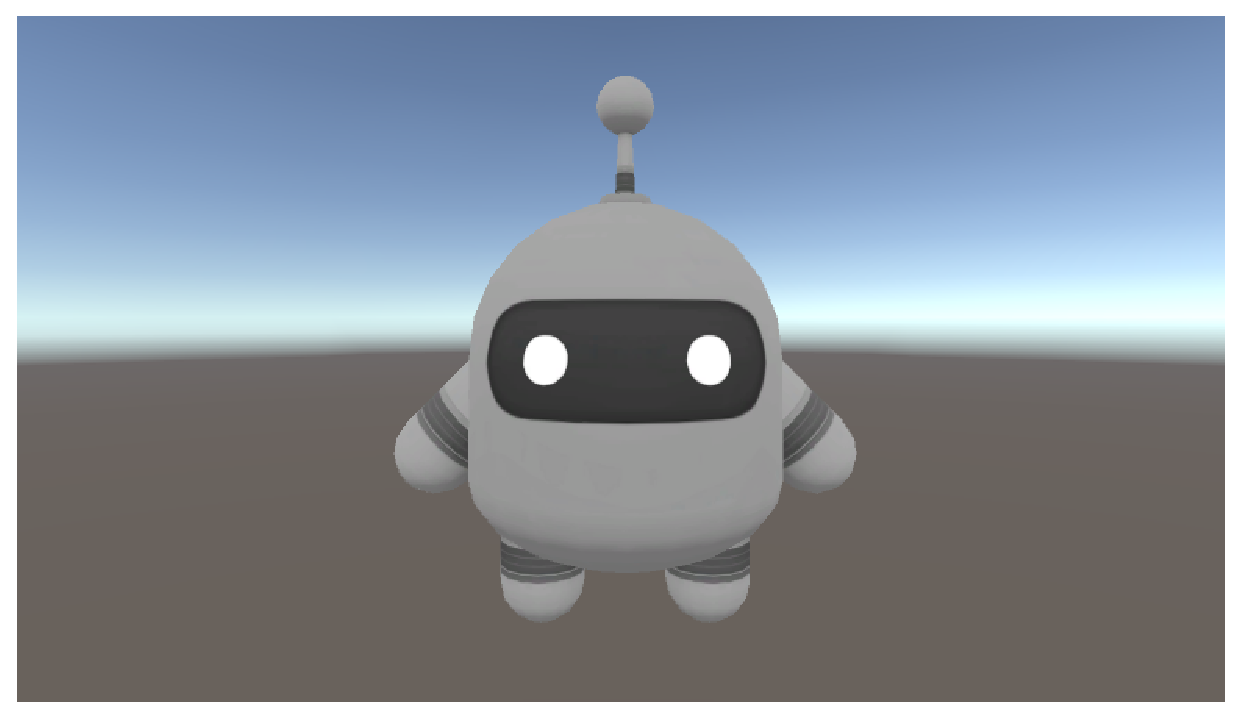
\includegraphics[width=12cm]{images/chapter3/Idle.eps}
  \caption{Idle状態のロボット}
  \label{Idle}
 \end{center}
\end{figure}

\vspace{1cm}
 \begin{figure}[!h]
 \begin{center}
  \centering
  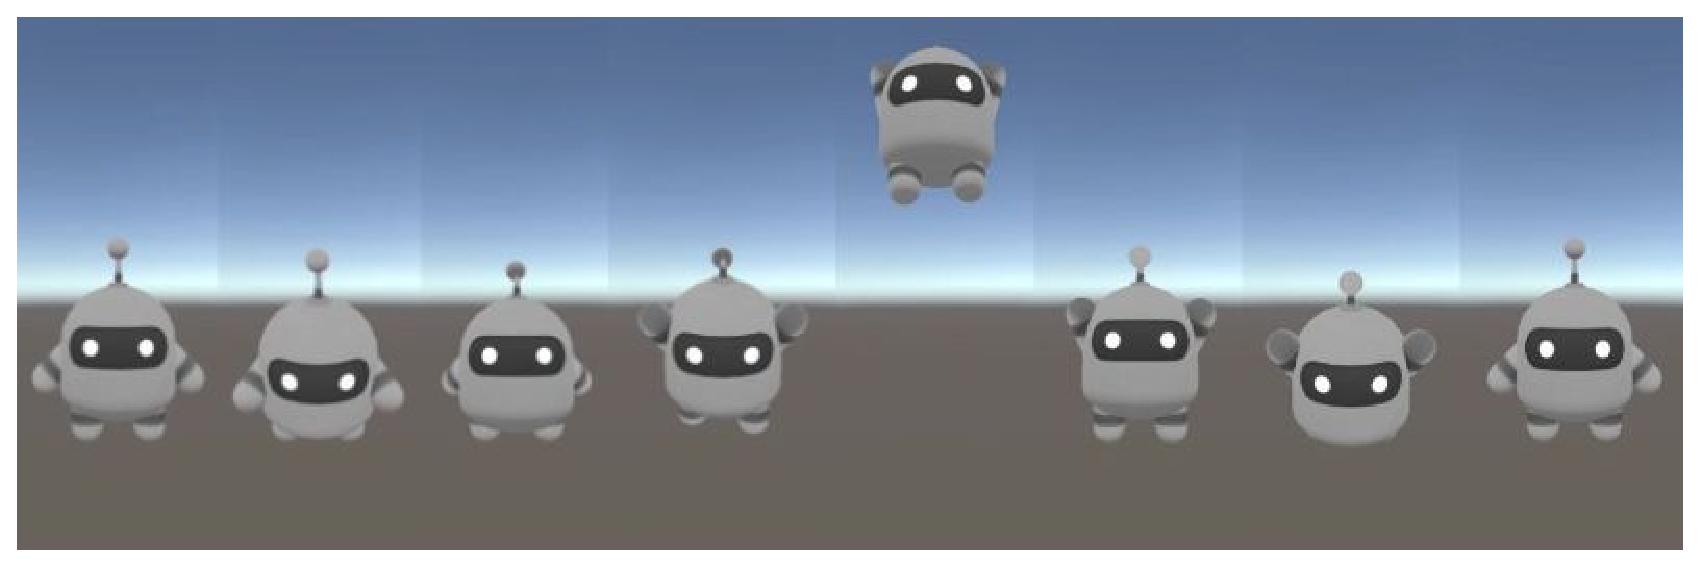
\includegraphics[width=12cm]{images/chapter3/happy.eps}
  \caption{喜の表出感情}
  \label{happy}
 \end{center}
\end{figure}

\vspace{1cm}
 \begin{figure}[!h]
 \begin{center}
  \centering
  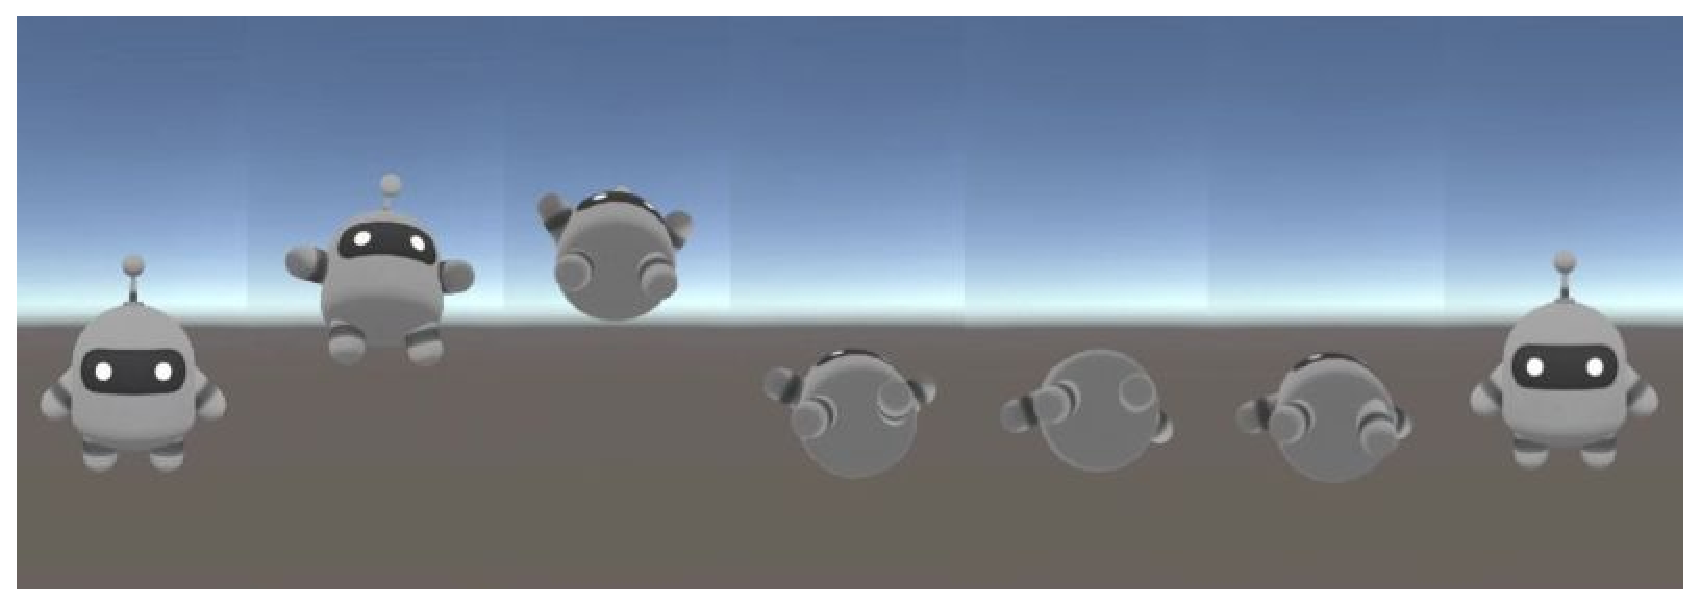
\includegraphics[width=12cm]{images/chapter3/sad.eps}
  \caption{哀の表出感情}
  \label{sad}
 \end{center}
\end{figure}

\newpage


















